\section{Estimating Speciation \& Extinction Rates Through Time}

\subsection{Outline}

This tutorial describes how to specify different models of incomplete taxon sampling \citep{Hoehna2011,Hoehna2014a} for estimating diversification rates in \RevBayes \citep{Hoehna2016b}.
Incomplete taxon sampling, if not modeled correctly, severely biases diversification-rate parameter estimates \citep{Cusimano2010,Hoehna2011}. 
Specifically, we will discuss \emph{uniform}, \emph{diversified}, and \emph{empirical} taxon sampling.
All analyses in this tutorial will focus on diversification rate estimation through-time and thus use a birth-death process where diversification rates vary episodically which we model by piecewise constant rates \RevBayes \citep{Hoehna2015a,May2016}.
The probabilistic graphical model is given only once for this tutorial as an overview.
The model itself does not change between the different analyses; only the assumptions of incomplete taxon sampling.
For each analysis you will estimate speciation and extinction rates through-time using Markov chain Monte Carlo (MCMC) and assess the impact of incomplete taxon sampling as well as the sampling scheme.


\subsection{Requirements}
We assume that you have read and hopefully completed the following tutorials:
\begin{itemize}
\item \href{https://github.com/revbayes/revbayes_tutorial/raw/master/tutorial_TeX/RB_Getting_Started/RB_Getting_Started.pdf}{Getting started}
\item \href{https://github.com/revbayes/revbayes_tutorial/raw/master/tutorial_TeX/RB_Basics_Tutorial/RB_Basics_Tutorial.pdf}{Rev basics}
\item \href{https://github.com/revbayes/revbayes_tutorial/raw/master/tutorial_TeX/RB_DiversificationRate_Tutorial/RB_DiversificationRate_Tutorial.pdf}{Basic Diversification Rate Estimation}
\item \href{https://github.com/revbayes/revbayes_tutorial/raw/master/tutorial_TeX/RB_DiversificationRate_Episodic_Tutorial/RB_DiversificationRate_Episodic_Tutorial.pdf}{Diversification Rates Through Time}
\end{itemize}
Note that the RB\_Basics\_Tutorial introduces the basic syntax of \Rev but does not cover any phylogenetic models.
You may skip the RB\_Basics\_Tutorial if you have some familiarity with \R.
We tried to keep this tutorial very basic and introduce all the language concepts and theory on the way.
You may only need the RB\_Basics\_Tutorial for a more in-depth discussion of concepts in \Rev.


%%%%%%%%
%%   Data   %%
%%%%%%%%
\section{Data and files}

We provide the data file(s) which we will use in this tutorial.
You may want to use your own data instead.
In the \cl{data} folder, you will find the following files
\begin{itemize}
\item \cl{primates.tre}: Dated primates phylogeny including 23 out of 377 species.
\end{itemize}
Note that we use here the small primate phylogeny including only 23 of the 377 taxa instead of the much more complete primate phylogeny from \cite{Springer2012}.
This choice was solely made to emphasize the point and impact of incomplete taxon sampling, which is a very prominent feature in many large scale phylogenies.

\impmark{Open the tree \cl{data/primates.tre} in \FigTree.}


\bigskip
\section{Episodic Birth-Death Model}

We study the impact of incomplete taxon sampling by estimating diversification rates through time.
The goal is to compare the impact of the sampling strategies rather than the description of the diversification-rate model itself.
The episodic birth-death model used here is equivalent to the model described in our previous tutorial.
Please read the \href{https://github.com/revbayes/revbayes_tutorial/raw/master/tutorial_TeX/RB_DiversificationRate_Episodic_Tutorial/RB_DiversificationRate_Episodic_Tutorial.pdf}{Diversification Rates Through Time} tutorial for more detailed information about the model.

\begin{figure}[h!]
\centering
\fbox{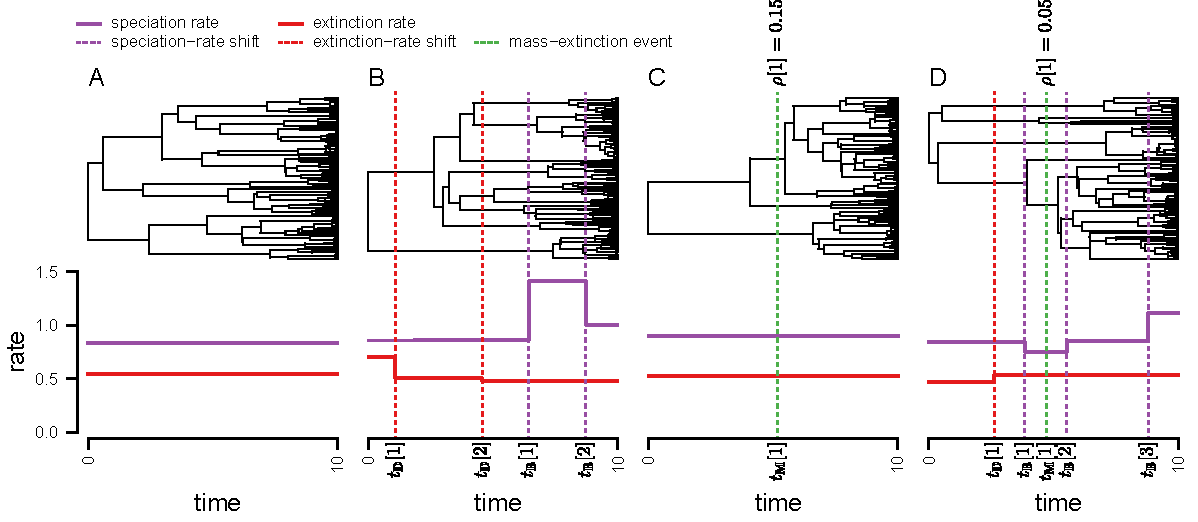
\includegraphics[width=\textwidth]{\ResourcePath figures/EBD_scenarios.pdf}}
\caption{\small Four scenarios of birth-death models.}
\label{fig:EBD}
\end{figure}



\subsection{Read the tree}

Begin by reading in the observed tree. 

{\tt \begin{snugshade*}
\begin{lstlisting}
T <- readTrees("data/primates.tre")[1]
\end{lstlisting}
\end{snugshade*}}

From this tree, we can get some helpful variables:
{\tt \begin{snugshade*}
\begin{lstlisting}
taxa <- T.taxa()
\end{lstlisting}
\end{snugshade*}}

Additionally, we can initialize an iterator variable for our vector of moves and another iterator variable for the number of monitors:
{\tt \begin{snugshade*}
\begin{lstlisting}
mvi = 0
mni = 0
\end{lstlisting}
\end{snugshade*}}

Finally, we create a helper variable that specifies the number of intervals.
{\tt \begin{snugshade*}
\begin{lstlisting}
NUM_INTERVALS = 20
\end{lstlisting}
\end{snugshade*}}
Using this variable we can easily change our script to break-up time into many or few intervals.



\subsection{Specifying the model}

\subsubsection{Priors on rates}
We start by specifying prior distributions on the rates.
Each interval-specific speciation and extinction rate will be drawn from a normal distribution.
Thus, we need a parameter for the standard deviation of those normal distributions.
We use an exponential hyperprior with rate 1.0 to estimate the standard deviation, but assume that all speciation rates and all extinction rates share the same standard deviation.
The motivation for an exponential hyperprior is that it has the highest probability density at 0 which would make he variance between rates 0 too and thus represent a constant rate process.
The data will tell us if there should be much variation in rates through time.
{\tt \begin{snugshade*}
\begin{lstlisting}
speciation_sd ~ dnExponential(1.0)
extinction_sd ~ dnExponential(1.0)
\end{lstlisting}
\end{snugshade*}}
We apply a simple scaling move on each prior parameter.
{\tt \begin{snugshade*}
\begin{lstlisting}
moves[++mvi] = mvScale(speciation_sd,weight=5.0)
moves[++mvi] = mvScale(extinction_sd,weight=5.0)
\end{lstlisting}
\end{snugshade*}}

The second prior parameter that we need to specify is the prior mean of the speciation and extinction rate at present.
This is because we are actually modeling rate-changes backwards in time and there is no previous rate for the rate at the present.
Thus we use a uniform distribution between -10 and 10 because of lack of prior knowledge.
{\tt \begin{snugshade*}
\begin{lstlisting}
# draw the mean from a uniform distribution
speciation_prior_mean ~ dnUniform(-10.0,10.0)
extinction_prior_mean ~ dnUniform(-10.0,10.0)
\end{lstlisting}
\end{snugshade*}}
This time we will apply a simple sliding window move because both parameters are location parameters instead of scale or variance parameters.
{\tt \begin{snugshade*}
\begin{lstlisting}
moves[++mvi] = mvSlide(speciation_prior_mean,weight=5.0)
moves[++mvi] = mvSlide(extinction_prior_mean,weight=5.0)
\end{lstlisting}
\end{snugshade*}}


\subsubsection{Specifying episodic rates}
As we mentioned before, we will apply normal distributions as priors for each rate.
We begin with the rate at the present.
The rates at the present will be specified slightly differently because they are not correlated to any previous rates.
Note that we store the variables in vectors.
{\tt \begin{snugshade*}
\begin{lstlisting}
log_speciation[1] ~ dnNormal( mean=speciation_prior_mean, sd=speciation_sd )
log_extinction[1] ~ dnNormal( mean=extinction_prior_mean, sd=extinction_sd )
\end{lstlisting}
\end{snugshade*}}
Again, we apply simple sliding window moves for the rates.
Normally we would use scaling moves but in this case we work on the log-transformed parameters and thus sliding moves perform better.
If you are keen you can test the differences.
{\tt \begin{snugshade*}
\begin{lstlisting}
moves[++mvi] = mvSlide(log_speciation[1], weight=2)
moves[++mvi] = mvSlide(log_extinction[1], weight=2)
\end{lstlisting}
\end{snugshade*}}
Now we transform the parameters.
{\tt \begin{snugshade*}
\begin{lstlisting}
speciation[1] := exp( log_speciation[1] )
extinction[1] := exp( log_extinction[1] )
\end{lstlisting}
\end{snugshade*}}

Then we repeat the specification for the speciation and extinction rates for each time interval.
This can be done efficiently using a \cl{for}-loop.
We will use a specific index variable so that we can easier refer to the rate at the previous interval.
{\tt \begin{snugshade*}
\begin{lstlisting}
for (i in 1:NUM_INTERVALS) {
    index = i+1
    
    log_speciation[index] ~ dnNormal( mean=log_speciation[i], sd=speciation_sd )
    log_extinction[index] ~ dnNormal( mean=log_extinction[i], sd=extinction_sd )

    moves[++mvi] = mvSlide(log_speciation[index], weight=2)
    moves[++mvi] = mvSlide(log_extinction[index], weight=2)

    speciation[index] := exp( log_speciation[index] )
    extinction[index] := exp( log_extinction[index] )

}
\end{lstlisting}
\end{snugshade*}}
Finally, we apply moves that slide all values in the vectors, \IE all speciation or extinction rates, by the same amount. 
This again considerably improves the efficiency of our MCMC analysis.
{\tt \begin{snugshade*}
\begin{lstlisting}
moves[++mvi] = mvVectorSlide(log_speciation, weight=10)
moves[++mvi] = mvVectorSlide(log_extinction, weight=10)
\end{lstlisting}
\end{snugshade*}}


\subsubsection{Setting up the time intervals}
In \RevBayes you actually have the possibility unequal time intervals or even different intervals for the speciation and extinction rate.
This is achieved by providing a vector of times when each interval ends.
Here we simply break-up the most recent 80\% of time since the root in equal intervals.
{\tt \begin{snugshade*}
\begin{lstlisting}
interval_times = T.rootAge() * (1:NUM_INTERVALS) / (NUM_INTERVALS) * 0.8
\end{lstlisting}
\end{snugshade*}}


\subsubsection{Incomplete Taxon Sampling}

We know that we have sampled 23 out of 377 living primate species. 
To account for this we can set the sampling parameter as a constant node with a value of 23/377.
Moreover, we assume that every taxon alive today had the same sampling probability, and thus, taxa were uniformly sampled at the present time.
This sampling scheme is called \emph{uniform} taxon sampling \citep{Hoehna2011,Hoehna2014a}.
{\tt \begin{snugshade*}
\begin{lstlisting}
rho <- T.ntips()/377
\end{lstlisting}
\end{snugshade*}}


\subsubsection{Root age}

The birth-death process requires a parameter for the root age.
In this exercise we use a fix tree and thus we know the age of the tree.
Hence, we can get the value for the root from the tree.
{\tt \begin{snugshade*}
\begin{lstlisting}
root_time <- T.rootAge()
\end{lstlisting}
\end{snugshade*}}

\subsubsection{The time tree}

Now we have all of the parameters we need to specify the full episodic birth-death model. 
We initialize the stochastic node representing the time tree.
{\tt \begin{snugshade*}
\begin{lstlisting}
timetree ~ dnEpisodicBirthDeath(rootAge=T.rootAge(), lambdaRates=speciation, lambdaTimes=interval_times, muRates=extinction, muTimes=interval_times, rho=rho, samplingStrategy="uniform", condition="time", taxa=taxa)
\end{lstlisting}
\end{snugshade*}}
And then we attach data to it.
{\tt \begin{snugshade*}
\begin{lstlisting}
timetree.clamp(T)
\end{lstlisting}
\end{snugshade*}}

Finally, we create a workspace object of our whole model using the \cl{model()} function. 
{\tt \begin{snugshade*}
\begin{lstlisting}
mymodel = model(speciation)
\end{lstlisting}
\end{snugshade*}}

The \cl{model()} function traversed all of the connections and found all of the nodes we specified. 


\subsection{Running an MCMC analysis}

\subsubsection{Specifying Monitors}

For our MCMC analysis, we need to set up a vector of \textit{monitors} to record the states of our Markov chain. 
First, we will initialize the model monitor using the \cl{mnModel} function. This creates a new monitor variable that will output the states for all model parameters when passed into a MCMC function. 
{\tt \begin{snugshade*}
\begin{lstlisting}
monitors[++mni] = mnModel(filename="output/primates_uniform.log",printgen=10, separator = TAB)
\end{lstlisting}
\end{snugshade*}}

Additionally, we create four separate file monitors, one for each vector of speciation and extinction rates and for each speciation and extinction rate epoch (\IE the times when the interval ends).
We want to have the speciation and extinction rates stored separately so that we can plot them nicely afterwards.
{\tt \begin{snugshade*}
\begin{lstlisting}
monitors[++mni] = mnFile(filename="output/primates_uniform_speciation_rates.log",printgen=10, separator = TAB, speciation)
monitors[++mni] = mnFile(filename="output/primates_uniform_speciation_times.log",printgen=10, separator = TAB, interval_times)
monitors[++mni] = mnFile(filename="output/primates_uniform_extinction_rates.log",printgen=10, separator = TAB, extinction)
monitors[++mni] = mnFile(filename="output/primates_uniform_extinction_times.log",printgen=10, separator = TAB, interval_times)
\end{lstlisting}
\end{snugshade*}}

Finally, create a screen monitor that will report the states of specified variables to the screen with \cl{mnScreen}:
{\tt \begin{snugshade*}
\begin{lstlisting}
monitors[++mni] = mnScreen(printgen=1000, speciation_prior_mean, extinction_prior_mean, speciation_sd, extinction_sd)
\end{lstlisting}
\end{snugshade*}}

\subsubsection{Initializing and Running the MCMC Simulation}

With a fully specified model, a set of monitors, and a set of moves, we can now set up the MCMC algorithm that will sample parameter values in proportion to their posterior probability. The \cl{mcmc()} function will create our MCMC object:
{\tt \begin{snugshade*}
\begin{lstlisting}
mymcmc = mcmc(mymodel, monitors, moves)
\end{lstlisting}
\end{snugshade*}}

First, we will run a pre-burnin to tune the moves and to obtain starting values from the posterior distribution.
{\tt \begin{snugshade*}
\begin{lstlisting}
mymcmc.burnin(generations=10000,tuningInterval=200)
\end{lstlisting}
\end{snugshade*}}


Now, run the MCMC:
{\tt \begin{snugshade*}
\begin{lstlisting}
mymcmc.run(generations=50000)
\end{lstlisting}
\end{snugshade*}}

When the analysis is complete, you will have the monitored files in your output directory.
You can then visualize the rates through time using \R using our package \RevGadgets.
If you don't have the R-package \RevGadgets installed, or if you have trouble with the package, then please read the separate tutorial about the package.

Just start \R in the main directory for this analysis and then type the following commands:
{\tt \begin{snugshade*}
\begin{lstlisting}
library(RevGadgets)

tree <- read.nexus("data/primates.tre")
files <- c("output/primates_uniform_speciation_times.log", "output/primates_uniform_speciation_rates.log", "output/primates_uniform_extinction_times.log", "output/primates_uniform_extinction_rates.log")

rev_out <- rev.process.output(files,tree,burnin=0.25,numIntervals=100)

pdf("uniform.pdf")
par(mfrow=c(2,2))
rev.plot.output(rev_out)
dev.off()
\end{lstlisting}
\end{snugshade*}}

\impmark{The \Rev file for performing this analysis: \href{https://github.com/revbayes/revbayes_tutorial/raw/master/RB_DiversificationRate_Sampling_Tutorial/scripts/mcmc_uniform.Rev}{\cl{mcmc\_uniform.Rev}}.}

\begin{figure}[h!]
\centering
\fbox{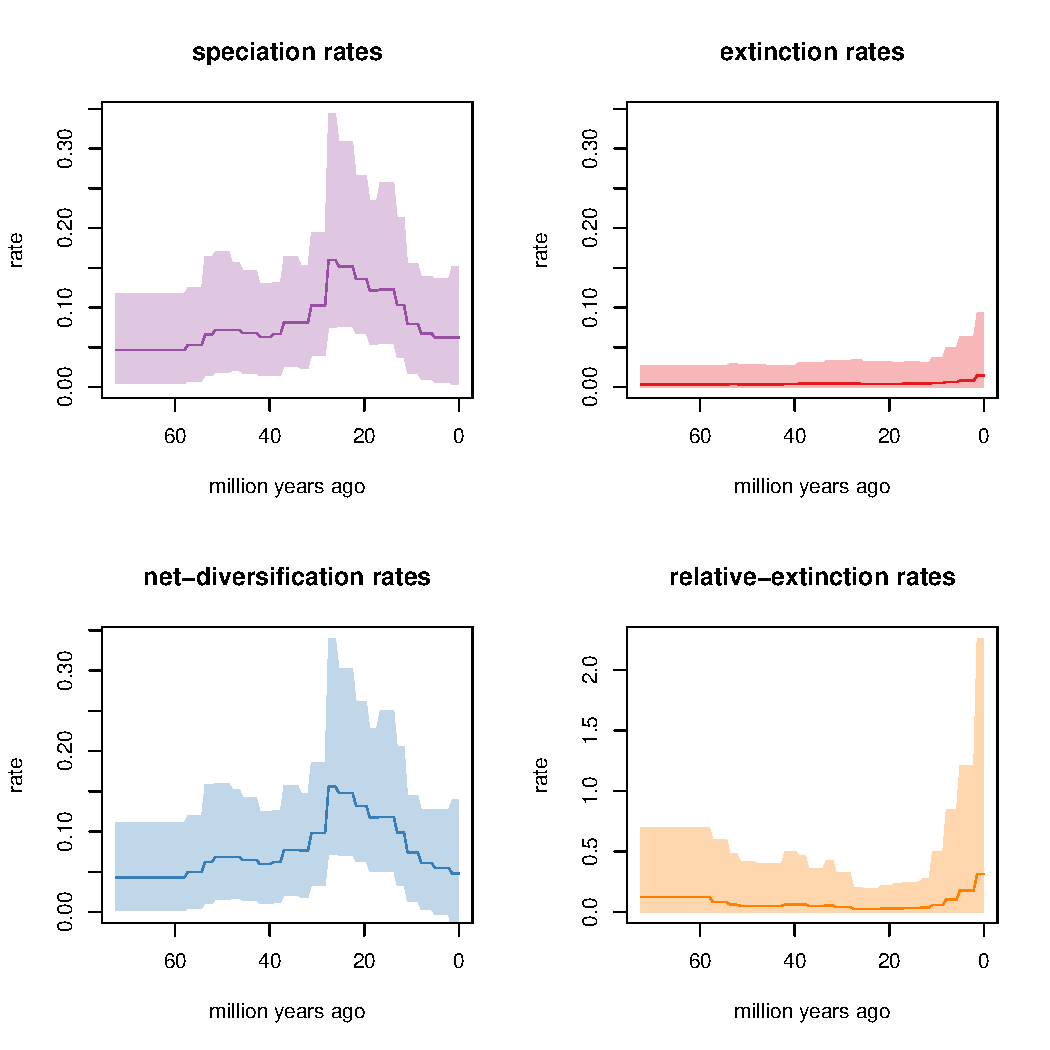
\includegraphics[width=\textwidth]{\ResourcePath figures/uniform.pdf}}
\caption{\small Resulting diversification rate estimations when using 20 intervals and assuming uniform taxon sampling. You should create similar plots for the other sampling schemes and compare the rates through time.}
\label{fig:EBD_Results}
\end{figure}

\subsection{Exercise}

\begin{itemize}
\item Run an MCMC simulation to estimate the posterior distribution of the speciation rate and extinction rate.
\item Visualize the rate through time using \R.
\end{itemize}



\newpage
\section{Diversified Taxon Sampling}

In the previous analysis we assumed that species were sampled uniformly.
However, this assumption is very often violated \citep{Hoehna2011}.
For example, the primate phylogeny that we use in this tutorial includes one species for almost all genera.
Thus, we had selected the species for the study not randomly but instead by including one species per genera and hence maximizing diversity.
This sampling scheme is called \emph{diversified} taxon sampling \citep{Hoehna2011}.

Figure~\ref{fig:DiversifiedSampling} shows an example of diversified sampling.
The example shows the same tree as in Figure~\ref{fig:BDP} where 5 species are sampled.
In fact, here we sampled 5 species so that every group is included and the most recent speciation events are excluded (not sampled).

\begin{figure}[h!]
\centering
\fbox{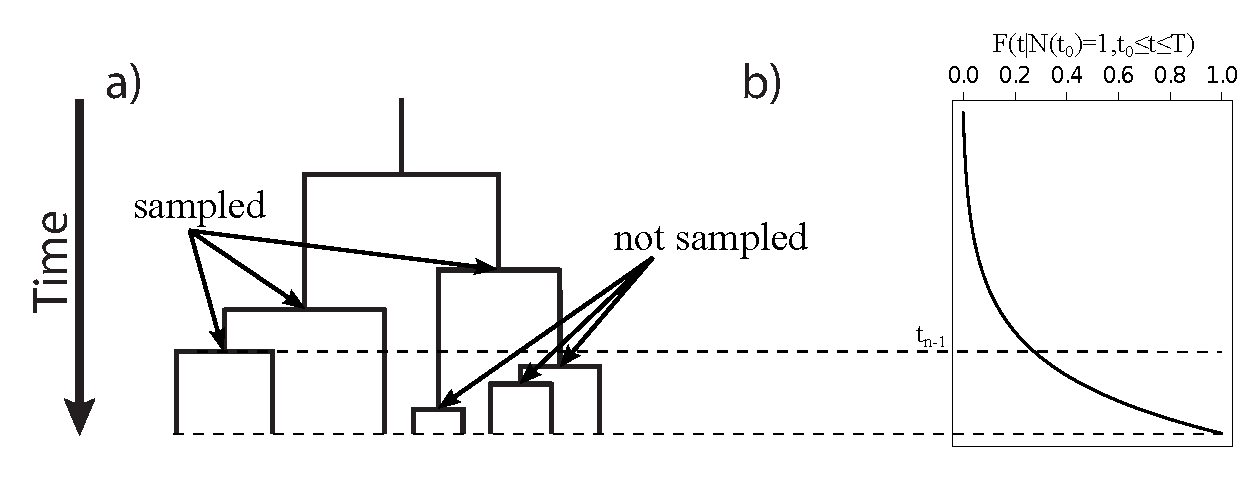
\includegraphics[width=\textwidth]{\ResourcePath figures/diversified-sampling.pdf}}
\caption{\small Example of diversified taxon sampling. a) An example phylogeny showing that all species after a certain time are not sampled. b) The cumulative probability of a speciation event occurring as a function of time. Here we see that the highest probability for a speciation event is more recently.}
\label{fig:DiversifiedSampling}
\end{figure}

{\tt \begin{snugshade*}
\begin{lstlisting}
timetree ~ dnEpisodicBirthDeath(rootAge=T.rootAge(), lambdaRates=speciation, lambdaTimes=interval_times, muRates=extinction, muTimes=interval_times, rho=rho, samplingStrategy="diversified", condition="time", taxa=taxa)
\end{lstlisting}
\end{snugshade*}}


\newpage
\section{Empirical Taxon Sampling}

Unfortunately, \emph{diversified} taxon sampling was derived under a strict mathematical concept that all species that speciated before a given time were included and all other species were discarded (not sampled); see Figure~\ref{fig:DiversifiedSampling}.
The \emph{diversified} sampling strategy is clearly to restrictive to be realistic and can bias parameter estimates too \citep{Hohna2014a}.
As another alternative we apply an \emph{empirical} taxon sampling strategy that uses empirical information on the clade relationships and speciation times of the missing species.
For example, in the primate phylogeny we know the crown age of the Hominoidea and know that 19 additional speciation events must have happened between the crown age of the Hominoidea and the present time to accommodate the 19 missing species (see Figure~\ref{fig:EmpiricalSampling}).
In fact, we can obtain for all larger groups the crown ages and the number of missing species and thus narrow down with empirical evidence the times when these missing speciation events have happened.

\begin{figure}[h!]
\centering
\fbox{
\includegraphics[width=\textwidth]{\ResourcePath figures/primates.png}}
\caption{\small Example of empirical taxon sampling. }
\label{fig:EmpiricalSampling}
\end{figure}

In the birth-death model we include these missing speciation events by integrating over the known interval when these have happened (between the crown age and the present).
This integral of the probability density of a speciation event is exactly the same as one minus the cumulative distribution function of a speciation event, 
\begin{equation}
F(t|N(t_1)=1,t_1\leq t \leq T) = 1 - \frac{1-P(N(T)>0|N(t)=1)\exp{(r(t,T))}}{1-P(N(T)>0|N(t_1)=1)\exp{(r(t_1,T))}} \label{spec_dist}
\end{equation}
which was previously derived by \citet[Equation~(6)]{Hoehna2014a} (see also \citet[Equation~(3)]{Yang1997} for constant rates and \citet[Equation~(8)]{Hoehna2013}).

Thus, the joint probability density of the sampled reconstructed tree and the empirically informed missing speciation times is
\begin{eqnarray}
f(\Psi,\mathbb{M}|N(t_1\!=\!0)\!=\!2,S(2,t_1\!=\!0,T))  & = & f(\Psi|N(t_1\!=\!0)\!=\!2,S(2,t_1\!=\!0,T)) \nonumber \\
& &  \times\prod_{i=1}^{k}\left(1-F(t|N(t_{M}[i])=1,t_{M}[i]\leq t \leq T)\right)^{m_i}  \nonumber\\ \label{eq:timesAndMissing}
\end{eqnarray}
We will use Equation~(\ref{eq:timesAndMissing}) as the likelihood function in our Bayesian analysis.


{\tt \begin{snugshade*}
\begin{lstlisting}
Galagidae             = clade("Galago_senegalensis",  "Otolemur_crassicaudatus", missing= 17)
Lorisidae             = clade("Perodicticus_potto", "Loris_tardigradus", "Nycticebus_coucang", missing=6)
Cheirogaleoidea       = clade("Cheirogaleus_major", "Microcebus_murinus", missing= 19)
Lemuridae             = clade("Lemur_catta", "Varecia_variegata_variegata", missing=17)
Lemuriformes          = clade(Lemuridae, Cheirogaleoidea, missing=29)
Atelidae_Aotidae      = clade("Alouatta_palliata", "Aotus_trivirgatus", missing=30)
NWM                   = clade(Atelidae_Aotidae,"Callicebus_donacophilus", "Saimiri_sciureus", "Cebus_albifrons", missing=93)
Hominoidea            = clade("Pan_paniscus", "Hylobates_lar", missing=19)
Cercopithecoidea      = clade("Colobus_guereza", "Macaca_mulatta", "Chlorocebus_aethiops", missing=60)
\end{lstlisting}
\end{snugshade*}}


{\tt \begin{snugshade*}
\begin{lstlisting}
missing_species_per_clade = v(Galagidae, Lorisidae, Cheirogaleoidea, Lemuridae, Lemuriformes, Atelidae_Aotidae, NWM, Hominoidea, Cercopithecoidea)
\end{lstlisting}
\end{snugshade*}}


{\tt \begin{snugshade*}
\begin{lstlisting}
timetree ~ dnEpisodicBirthDeath(rootAge=T.rootAge(), lambdaRates=speciation, lambdaTimes=interval_times, muRates=extinction, muTimes=interval_times, rho=1.0, taxa=taxa, incompleteClades=missing_species_per_clade, condition="time")
\end{lstlisting}
\end{snugshade*}}


\bibliographystyle{sysbio}
\bibliography{\GlobalResourcePath refs}
